\section{Orbit Characteristics}
\label{pruneOrbit}
The orbits are determined depending on the characteristics of the payload. Because the payload uses a low power laser this means that the orbits will have to be \ac{LEO} in order for the laser to get any photons to the receivers. The resulting design option tree can be found in figure \ref{fig:pruneOrbit}, page \pageref{fig:pruneOrbit}. Further pruning is not possible without a detailed analysis of the remaining options --- which will take place in the tradeoff.

\begin{figure}
\centering
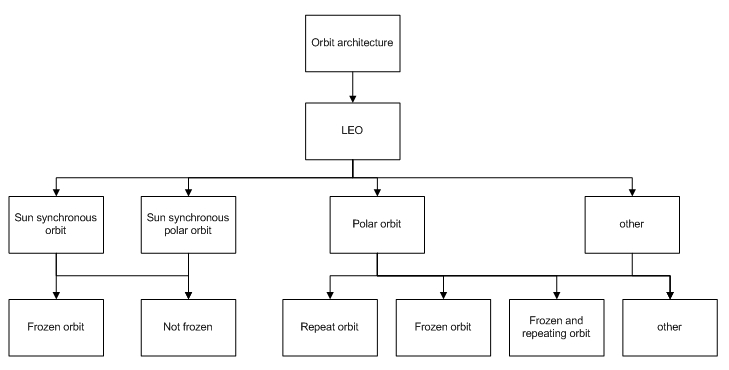
\includegraphics[width=0.8\textwidth, angle=0]{chapters/img/PrunedOrbit.jpg}
\label{fig:pruneOrbit}
\caption{Pruned design option tree for the orbit characteristics}
\end{figure}